\documentclass[a4paper, 11pt]{article}
\usepackage{geometry}
\usepackage{pdfpages}
\usepackage{graphicx}
\usepackage{blindtext}
\usepackage{amsmath}
\usepackage{listings}
\usepackage{xcolor}
\usepackage{floatrow}
\usepackage{subfig}
\usepackage{caption}
\usepackage{hyperref}

\geometry{
  top=35mm,
  bottom = 45mm
}

\definecolor{codegreen}{rgb}{0,0.6,0}
\definecolor{terminalbalck}{rgb}{0.3,0.3,0.3}
\definecolor{codegray}{rgb}{0.5,0.5,0.5}
\definecolor{codepurple}{rgb}{0.58,0,0.82}
\definecolor{backcolour}{rgb}{0.95,0.95,0.92}

\lstdefinestyle{terminal}{
    backgroundcolor=\color{terminalbalck},
    identifierstyle=\color{green},
    basicstyle=\ttfamily\footnotesize\color{green},
    showspaces=false,
    showstringspaces=false
}

\lstdefinestyle{code}{
    backgroundcolor=\color{backcolour},
    commentstyle=\color{codegreen},
    keywordstyle=\color{magenta},
    numberstyle=\tiny\color{codegray},
    stringstyle=\color{codepurple},
    basicstyle=\ttfamily\footnotesize,
    breakatwhitespace=false,
    breaklines=true,
    captionpos=b,
    keepspaces=true,
    numbers=left,
    numbersep=1pt,
    showspaces=false,
    showstringspaces=false,
    showtabs=false,
    tabsize=2
}

\begin{document}
  \title{Simulation of ALICE Project}
  \author{Coli Simone}
  \date{November 24th, 2021}
  \maketitle
  \section{Introduction}

  ALICE\_Simulation is a computer program that simulates the ALICE experiment that has been conducted at CERN since 1993, which consists of analyzing the collisions occurring between particles at very high energies$^{(1)}$. Those particles would create different particles following a probability distribution (Table\ref{table1}).
    \begin{table}[h!]
      \centering
      \begin{tabular}{ c c }
        \hline
        Particle Type & Probability \\
        \hline
        $\pi^+$ & $40\%$ \\
        $\pi^-$ & $40\%$ \\
        $k^+$ & $5\%$\\
        $k^-$ & $5\%$\\
        $P^+$ & $4.5\%$\\
        $P^-$ & $4.5\%$\\
        $k^*$ & $1\%$\\
        \hline
      \end{tabular}
      \caption{ \label{table1}
      \textit{The table shows the probability of obtaining a specific particle from a collision of high energy particles}
      }
    \end{table}\\

    In the simulation, we generated a finite amount of particles resulting from the collision of the flux in the particle accelerator, each with a proper momentum, mass, and resulting energy to maintain the conservation of those properties.The goal of the experiment is to detect the existence of the Kaon 0 ($k^*$), a very rare particle that decays into either a Positive Pion ($\pi^+$) and Negative Kaon ($k^-$) or a Negative Pion ($\pi^-$) and Positive Kaon ($k^+$), after only $5.2 \times 10^{-8}s$. We therefore stored the data of momentum, energy, charge, and invariant mass of all the particles to detect the presence of differences that could indicate the existence of the Kaon.

    The program we implemented stores the information about the particles and generates histograms from which we studied the system.
    \section{Code Structure}
      The code's division into different files and folders has the background idea of making it more orderly. There are eight files for the simulation program (one main file: \verb|mainE.cpp|, one libraries file: \verb|library.hpp|, three header files: \verb|ParticleType.hpp|, \verb|ResonanceType.hpp|, \verb|Particle.hpp|, and three source files: \verb|ParticleType.cpp|, \verb|Reso|- \verb|nanceType.cpp|, \verb|Particle.cpp|) and one for the data analysis (\verb|analysis.C|).
      The header files contain the classes implemented for the proper functioning of the simulation. Meanwhile, the source files contain the implementation of the methods defined in the headers.
      \subsection*{ParticleType Class}
      The class \verb|ParticleType| creates a homonymous type that contains the name, the mass, and the charge of a particular particle, respectively as a \verb|std::string|, a \verb|double|, and an \verb|integer|. This class has five methods, two of which are virtual.
      \subsection* {ResonanceType Class}
      The \verb|ResonanceType| class is a derived class from \verb|ParticleType| and, in addition to the base class items, it contains the information about the width of the particle as a double. The type defined with the name of this class creates a particle with a width. Contrarily to what happens for a \verb|ParticleType| object, in which the width of the particle is always zero. This class has two methods, both of them are the override of the already existing virtual methods in the base class.
      \subsection* {Particle Class}
      The class \verb|Particle| is the one that allows creating a particle giving it a random momentum and making it decay into other particles if necessary. It also creates a set of particles type, each with a proper index as an identifier. The variables in the class are three momentum components (\verb|fPx|, \verb|fPy|, \verb|fPz|), an array of ParticleType and its dimension (\verb|fParticleType|, \verb|fMaxNumParticleType|), an index of particle type (\verb|fNParticleType|), and a numeric code proper of each particle type \verb|fIndex|). This class has, also, several methods, including some static, which means they are accessible from the main without defining an object.
    \section{Generation}
      In the simulation, there had been 10000 collision events, each using a set of 100 particles. The particles resulting from the collisions were Positive Pions ($\pi^+$), Negative Pions ($\pi^-$), Positive Kaons ($k^+$), Negative Kaons ($k^-$), Protons ($p^+$), Antiprotons ($p^-$), and Resonance Kaons ($k^*$), generated randomly using a uniform distribution and the probability shown in Table 1.  The module of the momentum of the particles comes from an exponential distribution with a mean of 1. While its direction drives from the cartesian components:
      \begin{equation}
        \begin{cases}
          p_x = |p| \cdot \cos \theta \cdot \cos \phi\\
          p_y = |p| \cdot \cos \theta \cdot \sin \phi\\
          p_z = |p| \cdot \sin \theta
        \end{cases}
      \end{equation}\\
      Where the azimuthal angle theta ($\theta$) and the polar angle phi ($\phi$) are generated using a uniform random distribution respectively from 0 to $\pi$ and the second from 0 to $2\pi$.
      In the case that a Resonance Kaon is created from the collision of particles, it deacis into eather a Positive Pion and a Negative Kaon or a Negative Pion and a Positive Kaon with the same probability. The momentum of this new two particles comes from a normal distribution.
    \section{Analysis}
    The generation of particles types is compatible with the theoretical calculation as shown in Table. \ref{table2:Table 2}
    \begin{table}[h!]
      \centering
      \begin{tabular}{ c c c c }
        \hline
        Particle Type & Entries & Error & Theo. Ent. \\
        \hline
        $\pi^+$ & $3997740$ & $1999$ & $4\cdot10^6$\\
        $\pi^-$ & $4002160$ & $2001$ & $4\cdot10^6$\\
        $k^+$ & $500290$ & $707$ & $5\cdot10^5$\\
        $k^-$ & $499781$ & $707$ & $5\cdot10^5$\\
        $P^+$ & $449544$ & $671$ & $4.5\cdot10^5$\\
        $P^-$ & $450121$ & $671$ & $4.5\cdot10^5$\\
        $k^*$ & $100366$ & $317$ & $1\cdot10^5$\\
        \hline
      \end{tabular}
      \caption{ \label{table2:Table 2}
      \textit{The table shows the entries got from the simulation with the respective error calculated using root, and the theoretical entries calculated taking the percentage of each particle type from the total amount of particles.}
      }
    \end{table}\\
    As well as the angles and the momentum distributios are fitting the relative uniform and exponential distribution as shown in the images 1 and 2.
    \begin{figure}[h!]
      \centering
      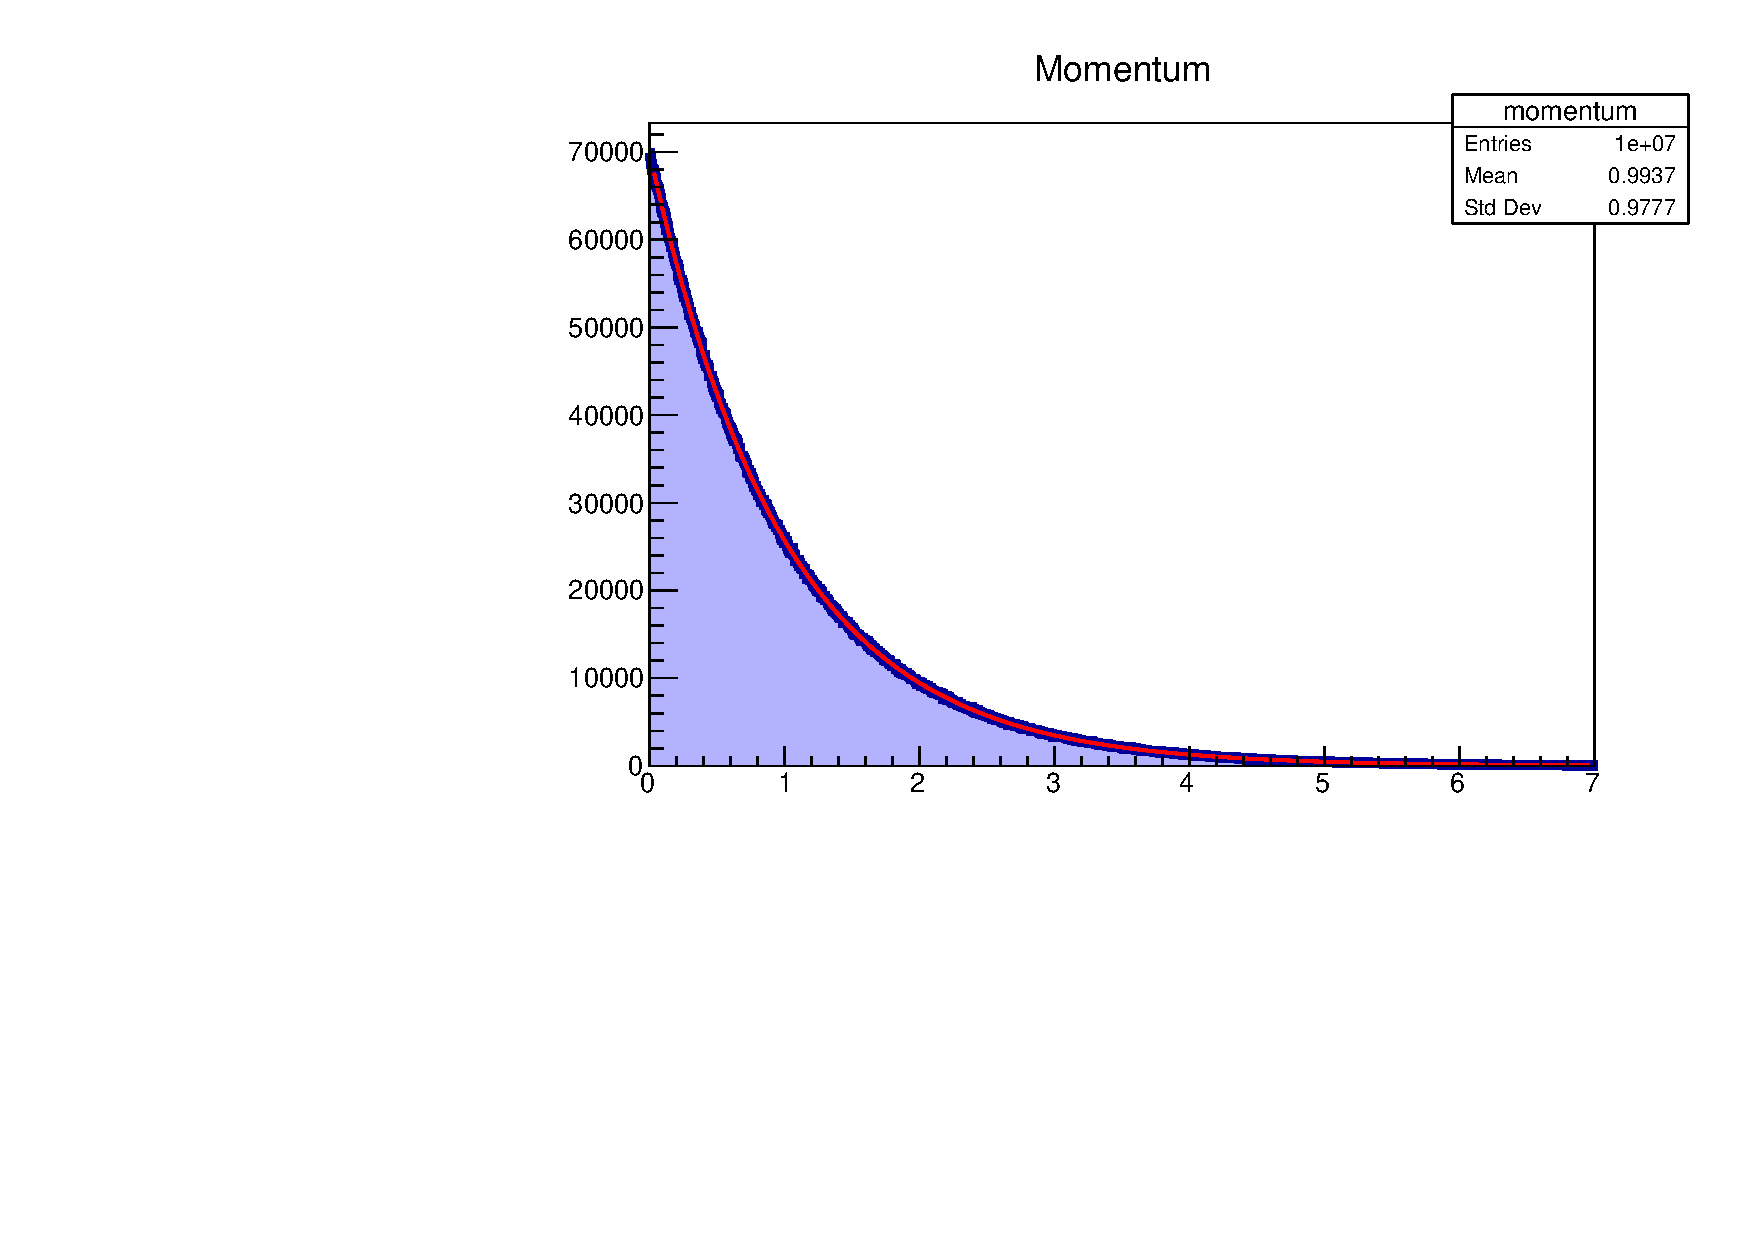
\includegraphics[width=9cm]{c1.pdf}
      \caption{\label{f1} \textit{The image shows the fit between the exponential distribution compared with the momentum histogram with occurrences randomly generated. The Chi-square divided by the number of degrees of freedom is very close to one, meaning that the histogram very well approximates an exponential distribution with a mean of 1.}}
    \end{figure}
    \begin{figure}
      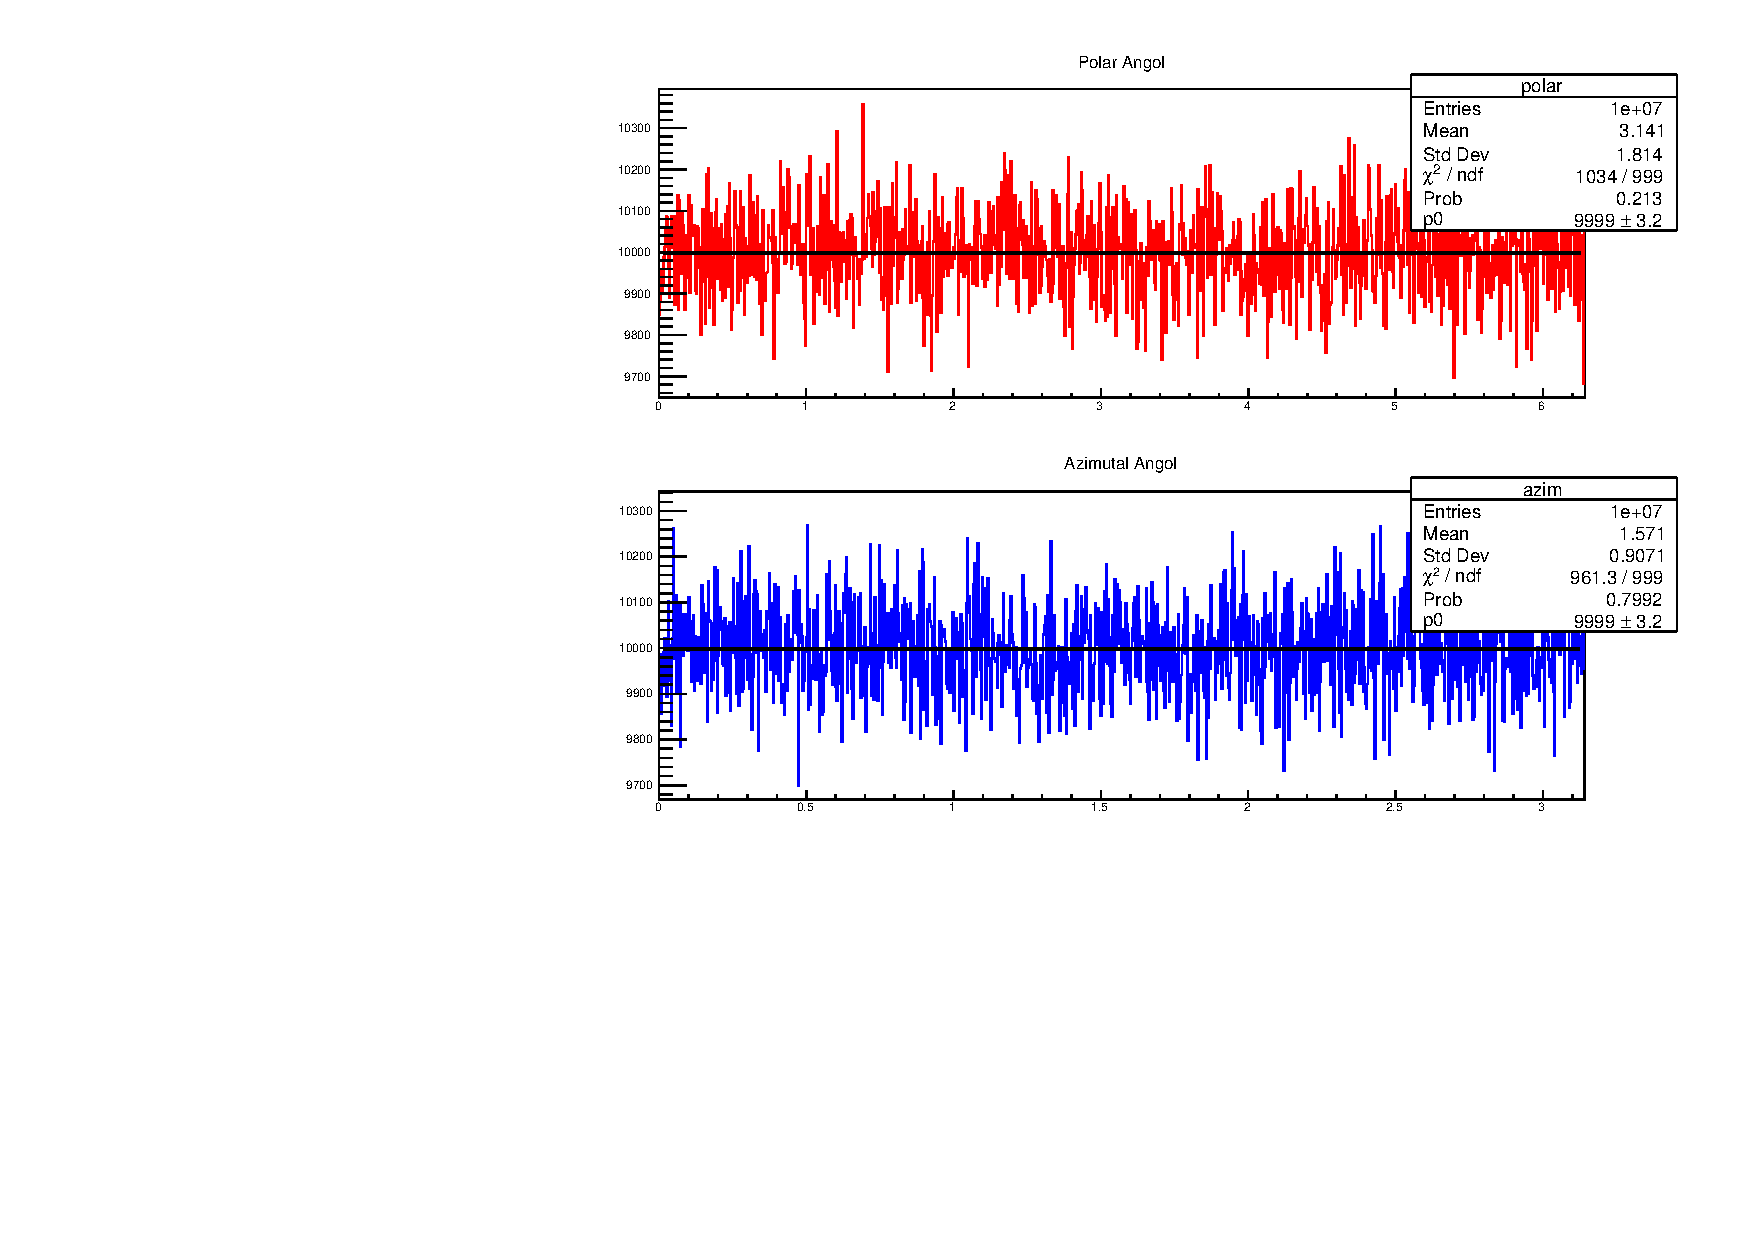
\includegraphics[width=9cm]{c2.pdf}
      \caption{\label{f2} \textit{The image shows the fit between the uniform distribution compared with the histogram of the angles randomly generated. The Chi-square divided by the number of degrees of freedom is very close to one, meanning that the histograms very well approximate an uniform distribution.}}
    \end{figure}
    \\
    It is possible to analyze these phenomena by looking at the histograms of the invariant mass. Because its definition contains both the momentum and the energy of the particles, we, therefore, assume it is conserved in the collision. Counting the number of particles per mass invariant value it is possible to construct the histogram of the invariant mass. The detection of the resonance Kaon consists of generating the histogram for only Pion and Kaon with different charges and comparing it with the histogram for the Pion and Kaon with the same charges. Because the resonance Kaon decays very quickly into those two particles with opposite charges, there should be a little "bump" in the first of those two histograms.
    \begin{figure}[h!]
      \centering
      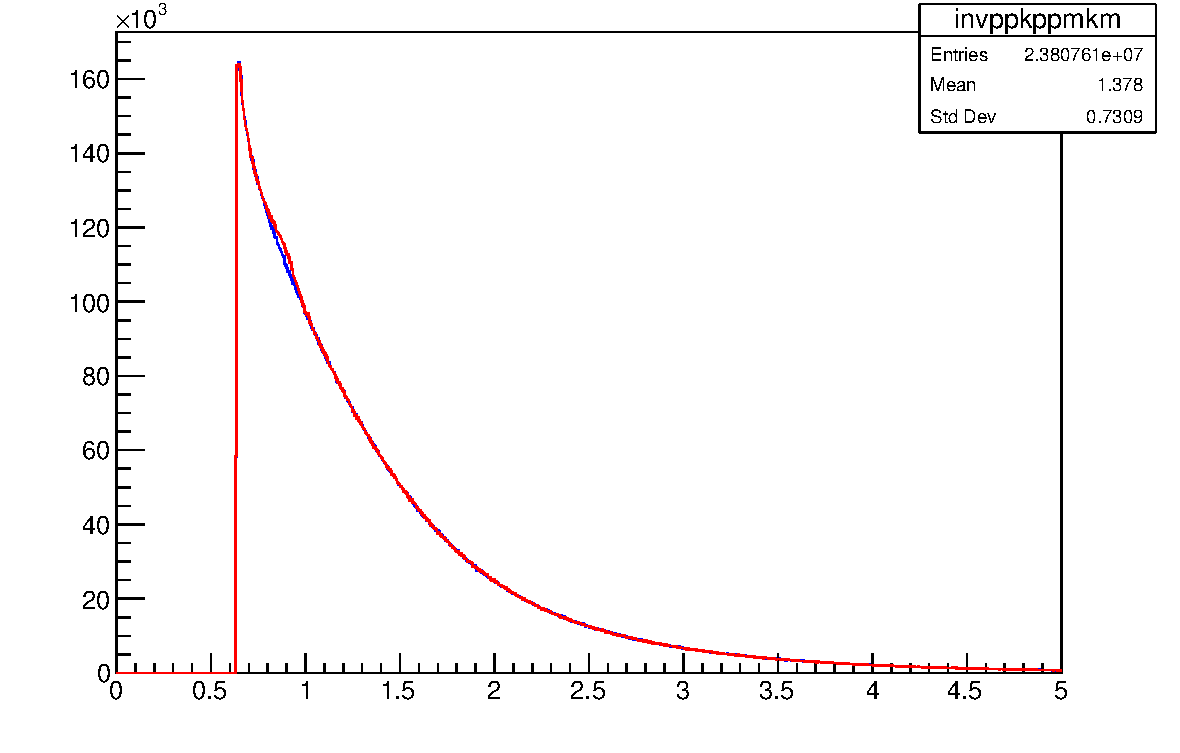
\includegraphics[width=9cm]{c4.pdf}
      \caption{\label{f3} \textit{The figure shows the histograms of the invariant mass in red and blue, respectively, of positive Pions \& negative kaons or negative Pions \& positive Kaons and positive Pions \& positive Kaons or negative Pions \& negative Kaons.}}
    \end{figure}\\
    A second approach consists of comparing the two histograms of the invariant mass of all the particles with the same charge and opposite charges.
    \\
    \begin{figure}[h!]
      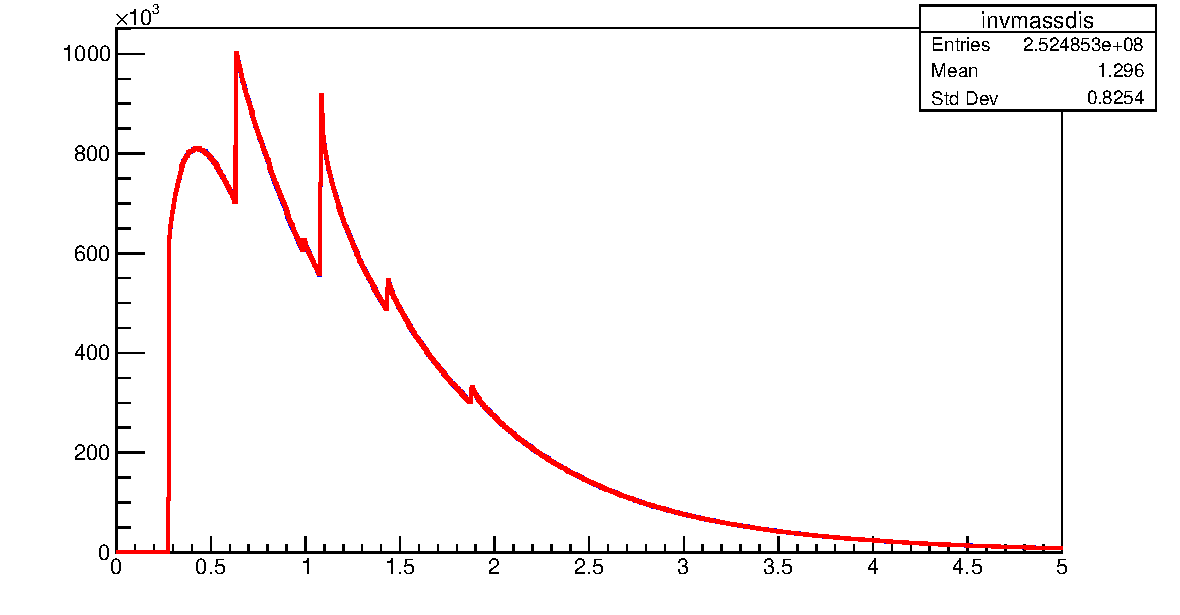
\includegraphics[width=9cm]{c3.pdf}
      \caption{\label{f4} \textit{The figure shows the two histograms of the invariant mass in red (thinnes) and blue (wider), respectively, of all the particles with same charges and all the particles with opposite charges.}}
    \end{figure}\\
    Subtracting the two pairs of histograms gives in both cases a bell shape, fitting a normal distribution with mean the mass of the resonance Kaon and sigma its error. Comparing the results with the testing histogram of the decay, filled during the simulation gives a very close value that stands inside the error.
    \\
    \begin{figure}[h!]
      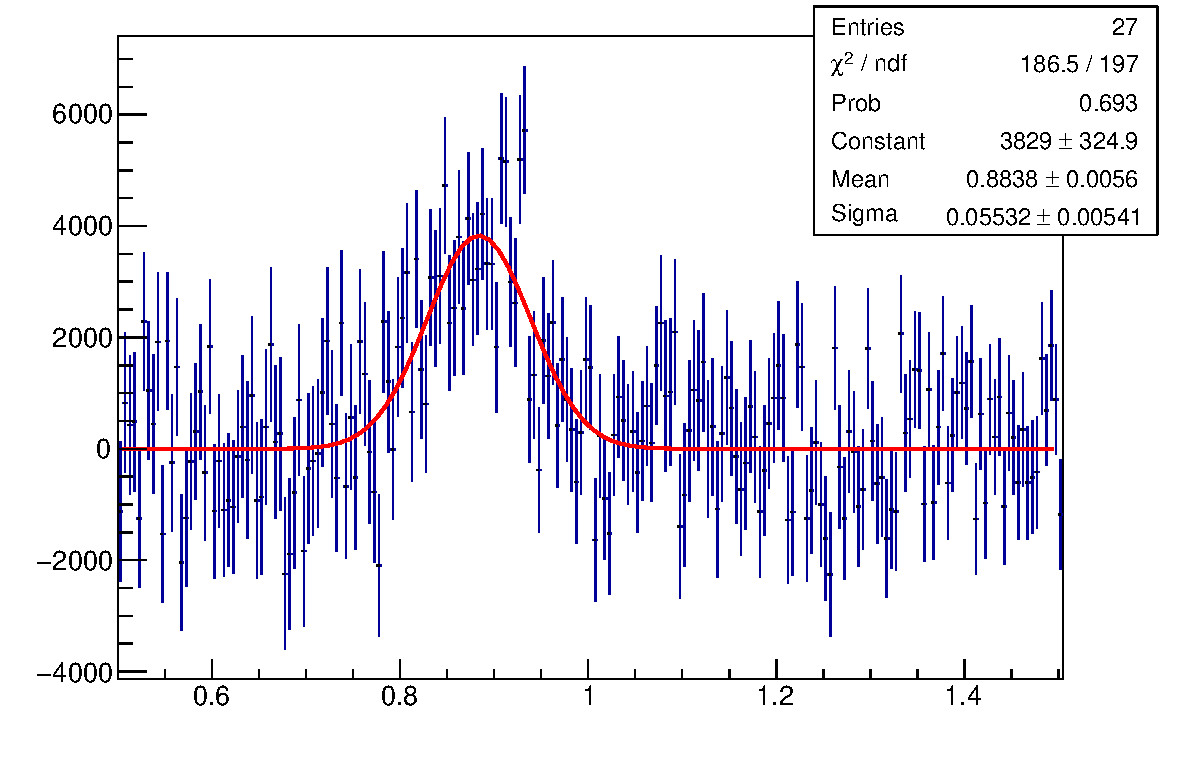
\includegraphics[width=9cm]{c6.pdf}
      \caption{\label{f5} \textit{The image shows the result of the subtraction between the histogram of the invariant mass of all the particles with the same charges and opposite charges. The red line represents the fitting normal distribution and the box shows the stats.}}
    \end{figure}
    \\
    \\
    \begin{figure}[h!]
      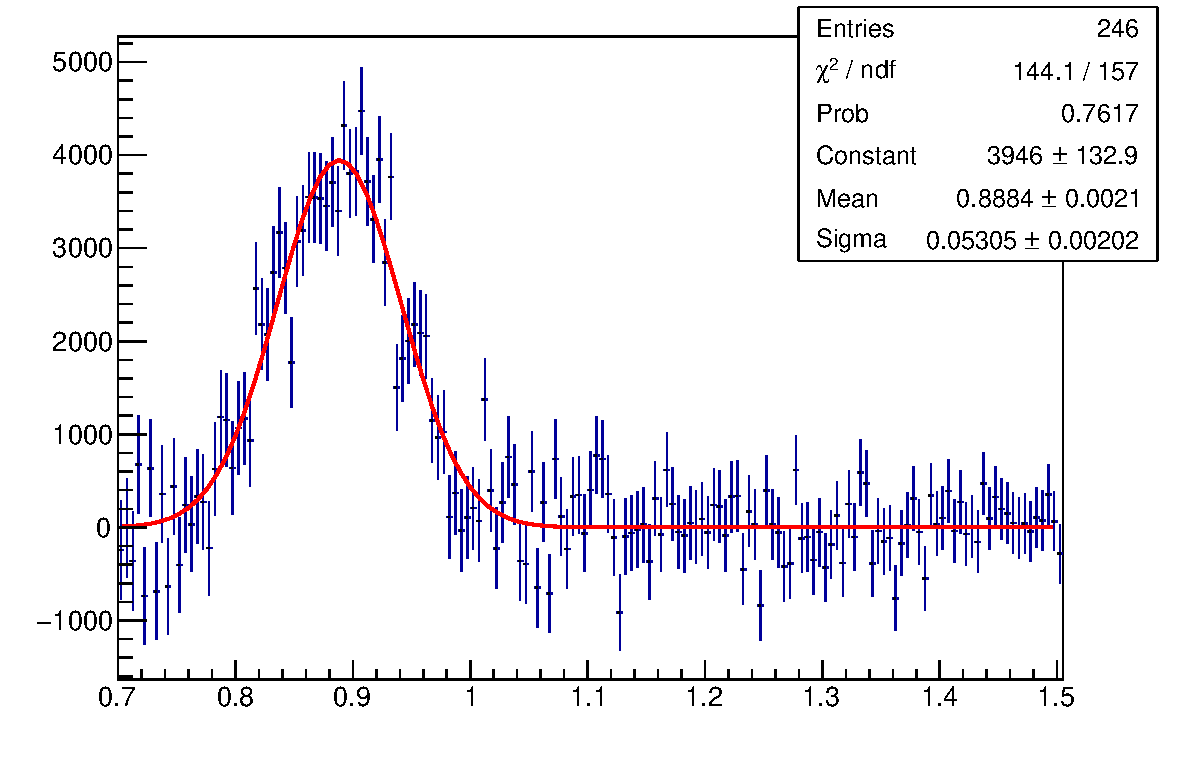
\includegraphics[width=9cm]{c5.pdf}
      \caption{\label{f6} \textit{This image show the result of the subtraction between the histogram of invariant mass of positive Pions \& negative kaons or negative Pions \& positive Kaon and the histogram of positive Pions \& positive Kaon or negative Pions \& negative Kaons. The red line represent the fitting normal distribution and the box shows its statts.}}
    \end{figure}
    \\
    In conclusion, the analysis of the first fit gives an experimental mass of $0.8838 \pm 0.0553$ Kg, while the second an experimental mass of $0.8884 \pm 0.0531$ Kg, both compatible with the supposed theoretical value of $0.89166$ Kg.

    \section{Code}
      \subsection{ParticleType.hpp}

        \begin{lstlisting}[language=c++, style=code]

  #ifndef PARTICLETYPE_HPP
  #define PARTICLETYPE_HPP

  #include <string>

  class ParticleType {
  private:
    const std::string fName;
    const double fMass;
    const int fCharge;
  public:

    //Constructor
    ParticleType(std::string Name, double Mass, int Charge);

    //Getters
    std::string GetParticleName() const;
    double GetParticleMass() const;
    int GetParticleCharge() const;
    virtual double GetParticleWidth() const;

    //Printer
    virtual void Print() const;
  };

  #endif
        \end{lstlisting}
      \subsection{ParticleType.cpp}
        \begin{lstlisting}[language=c++, style=code]

  #include <iostream>
  #include <string>
  #include "ParticleType.hpp"

  //Class ParticleType
  //----------------------
  //Constructor
  ParticleType::ParticleType(std::string Name, double Mass, int Charge):
  fName(Name),
  fMass(Mass),
  fCharge(Charge)
  {}

  //Getters
  std::string ParticleType::GetParticleName() const { return fName; }
  double ParticleType::GetParticleMass() const { return fMass; }
  int ParticleType::GetParticleCharge() const { return fCharge; }
  double ParticleType::GetParticleWidth() const { return 0; }


  //Printer
  void ParticleType::Print() const {
    std::cout << "Particle's Name: "<<fName << '\n';
    std::cout << "Particle's Mass: "<<fMass << '\n';
    std::cout << "Particle's Charge: "<<fCharge << '\n';
    std::cout << "-------------------------------------" << '\n';
  }
  //----------------------
        \end{lstlisting}
      \subsection{ResonanceType.hpp}
        \begin{lstlisting}[language=c++, style=code]

  #ifndef RESONANCETYPE_HPP
  #define RESONANCETYPE_HPP

  #include <string>
  #include "../ParticleType/ParticleType.hpp"

  class ResonanceType: public ParticleType {
  private:
    const double fWidth;
  public:

    //Constructor
    ResonanceType(std::string Name, double Mass, int Charge, double Width);

    //Pritner
    void Print() const;

    //Getter
    double GetParticleWidth() const;
  };

  #endif
        \end{lstlisting}
      \subsection{ResonanceType.cpp}
        \begin{lstlisting}[language=c++, style=code]

  #include <iostream>

  #include <string>
  #include "ResonanceType.hpp"

  //Class ResonanceType
  //----------------------
  //Constructor
  ResonanceType::ResonanceType(std::string Name, double Mass, int Charge, double Width):
  ParticleType(Name, Mass, Charge),
  fWidth(Width)
  {}

  //Getter
  double ResonanceType::GetParticleWidth() const { return fWidth; }

  //Printer
  void ResonanceType::Print() const {
    ParticleType::Print();
    std::cout << "Width of the Particle's Resonance: "<< fWidth << '\n';
  }
  //----------------------
        \end{lstlisting}
      \subsection{Particle.hpp}
        \begin{lstlisting}[language=c++, style=code]

  #ifndef PARTICLE_HPP
  #define PARTICLE_HPP

  #include <string>
  #include <vector>
  #include "../ParticleType/ParticleType.hpp"

  enum class PL{Electron, Positron, Proton, Antiproton, PionPlus, PionMinus, Pion0, KaonPlus, KaonMinus, Kaon0};

  class Particle {
  private:
    double fPx;
    double fPy;
    double fPz;

    static const int fMaxNumParticleType = 10;
    static ParticleType* fParticleType[fMaxNumParticleType];
    static int fNParticleType;
    int fIndex;

    static int FindParticle(std::string PTBF); //Particle To Be Found

    void Boost(double bx, double by, double bz);

  public:

    Particle(std::string name, double Px, double Py, double Pz);
    Particle() = default;
    static void AddParticle(std::string name , double mass , int charge , double with=0);
    static void AddParticle(PL particle);

    int GetIndex() const;
    int GetCharge() const;
    std::string GetName() const;
    double GetPx() const;
    double GetPy() const;
    double GetPz() const;
    double GetMass() const;
    double GetMomentum() const;
    double GetTotalEnergy() const;
    double GetInvMass(Particle& p) const;
    double GetTrasMomentum() const;

    void SetIndex(std::string);
    void SetIndex(int index);
    void SetMomentum(double x, double y, double z);

    static void PrintTable();
    void PrintParticle() const;

    static void ParticleFeatures(PL& particle, int const N);

    int Decay2body(Particle &dau1,Particle &dau2) const;


  };

  #endif
        \end{lstlisting}
      \subsection{Particle.cpp}
        \begin{lstlisting}[language=c++, style=code]

  #include "../../libraries/library.hpp"

  #include <string>
  #include <iostream>
  #include <cstdlib>
  #include <cmath>
  #include <random>

  int Particle::fNParticleType = 0;
  ParticleType* Particle::fParticleType[fMaxNumParticleType];

  // Public Methods //////////////////////////////////////
  int Particle::FindParticle(std::string PTBF) {
    int i = 0;
    for(; i < fNParticleType; ++i) {
      std::string ParticleName = fParticleType[i]->GetParticleName();
      if(ParticleName == PTBF) { return i; }
      else if (fNParticleType == 0) { return 0; }
    }
    return 10;
  }

  void Particle::AddParticle(std::string name, double mass, int charge, double width) {
    int const N = fNParticleType;
    int chack = FindParticle(name);
    if(N < fMaxNumParticleType && chack==10) {
      if(width!=0) {
        fParticleType[N] = new ResonanceType(name, mass, charge, width);
        ++fNParticleType;
      } else {
        fParticleType[N] = new ParticleType (name, mass, charge);
        ++fNParticleType;
      }
    } else {
      std::cout << "!! -- The particle Does alreay excist -- !!  " << '\n';
    }
  }

  int Particle::Decay2body(Particle &dau1,Particle &dau2) const {
    if(GetMass() == 0.0){
      printf("Decayment cannot be preformed if mass is zero\n");
      return 1;
    }

    double massMot = GetMass();
    double massDau1 = dau1.GetMass();
    double massDau2 = dau2.GetMass();

    if(fIndex < 10){ // add width effect

      // gaussian random numbers

      float x1, x2, w, y1, y2;

      double invnum = 1./RAND_MAX;
      do {
        x1 = 2.0 * rand()*invnum - 1.0;
        x2 = 2.0 * rand()*invnum - 1.0;
        w = x1 * x1 + x2 * x2;
      } while ( w >= 1.0 );

      w = sqrt( (-2.0 * log( w ) ) / w );
      y1 = x1 * w;
      y2 = x2 * w;
      massMot += fParticleType[fIndex]->GetParticleWidth() * y1;
    }
    if(massMot < massDau1 + massDau2){
      printf("Decayment cannot be preformed because mass is too low in this channel\n");
      return 2;
    }
    double pout = sqrt((massMot*massMot - (massDau1+massDau2)*(massDau1+massDau2))*(massMot*massMot - (massDau1-massDau2)*(massDau1-massDau2)))/massMot*0.5;
    double norm = 2*M_PI/RAND_MAX;
    double phi = rand()*norm;
    double theta = rand()*norm*0.5 - M_PI/2.;
    dau1.SetMomentum(pout*sin(theta)*cos(phi),pout*sin(theta)*sin(phi),pout*cos(theta));
    dau2.SetMomentum(-pout*sin(theta)*cos(phi),-pout*sin(theta)*sin(phi),-pout*cos(theta));
    double energy = sqrt(fPx*fPx + fPy*fPy + fPz*fPz + massMot*massMot);
    double bx = fPx/energy;
    double by = fPy/energy;
    double bz = fPz/energy;
    dau1.Boost(bx,by,bz);
    dau2.Boost(bx,by,bz);
    return 0;
  }

  void Particle::Boost(double bx, double by, double bz)
  {
    double energy = GetTotalEnergy();
    //Boost this Lorentz vector
    double b2 = bx*bx + by*by + bz*bz;
    double gamma = 1.0 / sqrt(1.0 - b2);
    double bp = bx*fPx + by*fPy + bz*fPz;
    double gamma2 = b2 > 0 ? (gamma - 1.0)/b2 : 0.0;

    fPx += gamma2*bp*bx + gamma*bx*energy;
    fPy += gamma2*bp*by + gamma*by*energy;
    fPz += gamma2*bp*bz + gamma*bz*energy;
  }

  // Constructor //////////////////////////////////////
  Particle::Particle(std::string name, double Px = 0, double Py = 0, double Pz = 0):
  fPx(Px),
  fPy(Py),
  fPz(Pz),
  fIndex (FindParticle(name))
  { if(fIndex == 10) { std::cout << "!! -- This Type of Particle does not Excist -- !!" << '\n'; } }

  // Getter Methods //////////////////////////////////////
  int Particle::GetIndex() const { return fIndex; }

  int Particle::GetCharge() const {return fParticleType[fIndex]->GetParticleCharge(); }

  std::string Particle::GetName() const {return fParticleType[fIndex]->GetParticleName();}

  double Particle::GetPx() const { return fPx; }

  double Particle::GetPy() const { return fPy; }

  double Particle::GetPz() const { return fPz; }

  double Particle::GetMass() const {
    return (fParticleType[fIndex]->GetParticleMass());
  }

  double Particle::GetMomentum() const {
    return (fPx*fPx + fPy*fPy + fPz*fPz);
  }

  double Particle::GetTrasMomentum() const {
    return fPx*fPx + fPy*fPy;
  }

  double Particle::GetTotalEnergy() const {
    double m = GetMass();
    double p2 = GetMomentum();
    return sqrt(m*m + p2);
  }

  double Particle::GetInvMass(Particle& p) const {
    double E1 = GetTotalEnergy();
    double E2 = p.GetTotalEnergy();
    double Psum = (fPx+p.GetPx())*(fPx+p.GetPx())+(fPy+p.GetPy())*(fPy+p.GetPy())+(fPz+p.GetPz())*(fPz+p.GetPz());
    double M = sqrt((E1+ E2)*(E1+ E2) - Psum);
    return M;
  }

  // Setter Methods //////////////////////////////////////
  void Particle::SetIndex(std::string type) {
    const int index = FindParticle(type);
    if(10 != index) {
      fIndex = index;
    }
  }

  void Particle::SetIndex(int index) {
    if(index < fNParticleType) {
      fIndex = index;
    }
  }

  void Particle::SetMomentum(double x, double y, double z) {
    fPx = x;
    fPy = y;
    fPz = z;
  }

  // Printer //////////////////////////////////////
  void Particle::PrintTable() {
    for(int i = 0; i < fNParticleType; ++i) {
      fParticleType[i]->Print();
    }
  }

  void Particle::PrintParticle() const {
    std::cout << "Particle index: " << fIndex << '\n';
    std::cout << "Particle name: "<< fParticleType[fIndex]->GetParticleName() << '\n';
    std::cout << "Px: "<< fPx << '\n';
    std::cout << "Py: "<< fPy << '\n';
    std::cout << "Pz: "<< fPz << '\n';
    std::cout << "-------------------------------------" << '\n';
  }

  // Particles List //////////////////////////////////////
  void Particle::ParticleFeatures(PL& particle, int const N) {
    int check;
    switch (particle) {
      case (PL::Electron):
        check = FindParticle("Electron");
        if (check == 10) {
          fParticleType[N] = new ParticleType ("Electron", 0.0005109, -1);
          ++fNParticleType;
        } else {
          std::cout << "!! -- The particle Does alreay excist -- !!  " << '\n';
        }
      break;
      case (PL::Proton) :
        check = FindParticle("Proton");
        if(check == 10) {
          fParticleType[N] = new ParticleType ("Proton", 0.938327, +1);
          ++fNParticleType;
        } else {
          std::cout << "!! -- The particle Does alreay excist -- !!  " << '\n';
        }
      break;
      case (PL::Positron) :
        check = FindParticle("Positron");
        if(check == 10) {
          fParticleType[N] = new ParticleType ("Positron", 0.0005109, +1);
          ++fNParticleType;
        } else {
          std::cout << "!! -- The particle Does alreay excist -- !!  " << '\n';
        }
      break;
      case (PL::PionMinus):
        check = FindParticle("Pion-");
        if(check == 10) {
          fParticleType[N] = new ParticleType ("Pion-", 0.13957, +1);
          ++fNParticleType;
        } else {
          std::cout << "!! -- The particle Does alreay excist -- !!  " << '\n';
        }
      break;
      case (PL::PionPlus) :
        check = FindParticle("Pion+");
        if(check == 10) {
          fParticleType[N] = new ParticleType ("Pion+", 0.13957, -1);
          ++fNParticleType;
        } else {
          std::cout << "!! -- The particle Does alreay excist -- !!  " << '\n';
        }
      break;
      case (PL::Pion0) :
        check = FindParticle("Pion0");
        if(check == 10) {
          fParticleType[N] = new ParticleType ("Pion0", 0.1350, 0);
          ++fNParticleType;
        } else {
          std::cout << "!! -- The particle Does alreay excist -- !!  " << '\n';
        }
      break;
      case (PL::KaonPlus) :
        check = FindParticle("Kaon+");
        if(check == 10) {
          fParticleType[N] = new ParticleType ("Kaon+", 0.49367, +1);
          ++fNParticleType;
        } else {
          std::cout << "!! -- The particle Does alreay excist -- !!  " << '\n';
        }
      break;
      case (PL::KaonMinus) :
        check = FindParticle("Kaon-");
        if(check == 10) {
          fParticleType[N] = new ParticleType ("Kaon-", 0.49367, -1);
          ++fNParticleType;
        } else {
          std::cout << "!! -- The particle Does alreay excist -- !!  " << '\n';
        }
      break;
      case (PL::Kaon0) :
        check = FindParticle("Kaon0");
        if(check == 10) {
          fParticleType[N] = new ResonanceType ("Kaon0", 0.89166, 0, 0.05);
          ++fNParticleType;
        } else {
          std::cout << "!! -- The particle Does alreay excist -- !!  " << '\n';
        }
      break;
      case (PL::Antiproton) :
        check = FindParticle("Antiproton");
        if(check == 10) {
          fParticleType[N] = new ParticleType ("Antiproton", 0.93827, -1);
          ++fNParticleType;
        } else {
          std::cout << "!! -- The particle Does alreay excist -- !!  " << '\n';
        }
      break;
      default:
        std::cout << "!! -- Particle not in the list, add it using the standard AddParticle -- !!" << '\n';
    }
  }

  void Particle::AddParticle(PL particle) {
    int const N = fNParticleType;
    ParticleFeatures(particle, N);
  }
        \end{lstlisting}
      \subsection{mainE.cpp}
        \begin{lstlisting}[language=c++, style=code]

  #include "../libraries/library.hpp"
  #include <iostream>
  #include <cmath>

  void ProgressionBar(int Progression) {
  double n = (Progression/5.22E8);
  std::cout << "[";
    int pos = 70 * n;
    for (int i = 0; i < 70; ++i) {
        if (i < pos) std::cout << "=";
        else if (i == pos) std::cout << ">";
        else std::cout << " ";
    }
    std::cout << "] " << int(n * 100.0) << " %\r";
    std::cout.flush();
  }

  int main() {
  double const pi = 3.1415926535;
  int progression = 0;
  TRandom* Random = new TRandom();
  Random->SetSeed(0);

  Particle::AddParticle(PL::PionPlus);
  Particle::AddParticle(PL::PionMinus);
  Particle::AddParticle(PL::KaonPlus);
  Particle::AddParticle(PL::KaonMinus);
  Particle::AddParticle(PL::Proton);
  Particle::AddParticle(PL::Antiproton);
  Particle::AddParticle(PL::Kaon0);

  TH1F* type = new TH1F("type", "Particles Type", 7, 0, 7);
  type->GetXaxis()->TAxis::SetBinLabel(1, "Pion+");
  type->GetXaxis()->TAxis::SetBinLabel(2, "Pion-");
  type->GetXaxis()->TAxis::SetBinLabel(3, "Kaon+");
  type->GetXaxis()->TAxis::SetBinLabel(4, "kaon-");
  type->GetXaxis()->TAxis::SetBinLabel(5, "Proton");
  type->GetXaxis()->TAxis::SetBinLabel(6, "Antiproton");
  type->GetXaxis()->TAxis::SetBinLabel(7, "Kaon0");

  TH1F* momentum = new TH1F("momentum", "Momentum", 1000, 0, 7);
  TH1F* tmomentum = new TH1F("tmomentum", "Transversal Momentum", 1000, 0, 7);
  TH1F* invmass = new TH1F("invmass", "Invarian Mass", 1000, 0, 5);
  TH1F* energy = new TH1F("energy","Energy", 1000, 0, 7);
  TH1F* azim = new TH1F("azim", "Azimutal Angol", 1000, 0, pi);
  TH1F* polar = new TH1F("polar", "Polar Angol", 1000, 0, 2*pi);
  TH1F* invmassdis = new TH1F("invmassdis", "Invariant Mass opposite charges", 1000, 0, 5);
  TH1F* invmasscon = new TH1F("invmasscon", "Invariant Mass same charges", 1000, 0, 5);
  TH1F* invppkmpmkp = new TH1F("invppkmpmkp", "Invariant Mass pion+/kaon- & pion-/kaon+", 1000, 0, 5);
  //invariant (i) mass (m) of pion (p) plus (p) and kaon (k) minus (m) or pion (p) minus (m) and kaon (k) plus (p)
  //i-m-p-p-k-m-p-m-k-p
  invppkmpmkp->SetLineColor(kRed);
  TH1F* invppkppmkm = new TH1F("invppkppmkm", "Invariant Mass pion+/kaon+ & pion-/kaon-", 1000, 0, 5);
  //invariant (i) mass (m) of pion (p) minus (m) and kaon (k) plus (p) or pion (p) minus (m) and kaon (k) minus (k)
  //i-m-p-p-k-p-p-m-k-m
  invppkppmkm->SetLineColor(kBlue);
  TH1F* decay = new TH1F("decay", "Invairant mass of particles from the decay", 1000, 0, 5);

  invmass->Sumw2();
  invmassdis->Sumw2();
  invmasscon->Sumw2();
  invppkmpmkp->Sumw2();
  invppkppmkm->Sumw2();
  decay->Sumw2();

  int const N = 100;
  int const extra = 20;
  Particle Particella[N+extra];

  for(int i = 0; i < 1E5; ++i) {
    int ExtraCounter = 0;
    for(int j = 0; j < (N); ++j) {

      double phi = 2*pi*Random->Uniform(0.0,1.0);
      double theta = pi*Random->Uniform(0.0,1.0);

      azim->Fill(theta);
      polar->Fill(phi);

      double P = Random->Exp(1.0);

      double Px = P*cos(phi)*cos(theta);
      double Py = P*cos(phi)*sin(theta);
      double Pz = P*sin(phi);

      Particella[j].SetMomentum(Px, Py, Pz);

      //Setting the type ///////////////////////////
      double prob = Random->Uniform(0.0,100.0);

      if(prob<40) {
        Particella[j].SetIndex("Pion+");
      } else if (prob<80) {
        Particella[j].SetIndex("Pion-");
      } else if (prob<85) {
        Particella[j].SetIndex("Kaon+");
      } else if (prob<90) {
        Particella[j].SetIndex("Kaon-");
      } else if (prob<94.5) {
        Particella[j].SetIndex("Proton");
      } else if (prob<99) {
        Particella[j].SetIndex("Antiproton");
      } else {
        Particella[j].SetIndex("Kaon0");
        int c = ExtraCounter + N;
        double chance = Random->Uniform(0.0,1.0);
        if(chance < 0.5) {
          Particella[c].SetIndex("Pion+");
          Particella[c+1].SetIndex("Kaon-");
        } else {
          Particella[c].SetIndex("Pion-");
          Particella[c+1].SetIndex("Kaon+");
        }
        int check = Particella[j].Decay2body(Particella[c], Particella[c+1]);
        if (check != 0) return check;
        double MassInvCondition = Particella[c].GetInvMass(Particella[c+1]);
        decay->Fill(MassInvCondition);
        ExtraCounter = ExtraCounter +2;
      }
      int index = Particella[j].GetIndex();
      type->Fill(index);
      double PTModule = sqrt(Particella[j].GetTrasMomentum());
      tmomentum->Fill(PTModule);
      double PModule = sqrt(Particella[j].GetMomentum());
      momentum->Fill(PModule);
      double Energy = Particella[j].GetTotalEnergy();
      energy->Fill(Energy);
      ++progression;
    }
    double MassInv;
   for(int k = 0; k <N+ExtraCounter; ++k) {
     for(int h = k+1 ; h<N+ExtraCounter; ++h){
       MassInv = Particella[k].GetInvMass(Particella[h]);
       invmass->Fill(MassInv);
       if((Particella[k].GetCharge() * Particella[h].GetCharge()) < 0) {
         double MassInvCondition = Particella[k].GetInvMass(Particella[h]);
         invmassdis->Fill(MassInvCondition);
       } else if((Particella[k].GetCharge() * Particella[h].GetCharge()) > 0) {
         double MassInvCondition = Particella[k].GetInvMass(Particella[h]);
         invmasscon->Fill(MassInvCondition);
       }
       if (Particella[k].GetName() == "Pion+" && Particella[h].GetName() == "Kaon-") {
         double MassInvCondition = Particella[k].GetInvMass(Particella[h]);
         invppkmpmkp->Fill(MassInvCondition);
       } else if(Particella[k].GetName() == "Pion-" && Particella[h].GetName() == "Kaon+") {
         double MassInvCondition = Particella[k].GetInvMass(Particella[h]);
         invppkmpmkp->Fill(MassInvCondition);
       } else if (Particella[k].GetName() == "Pion+" && Particella[h].GetName() == "Kaon+") {
         double MassInvCondition = Particella[k].GetInvMass(Particella[h]);
         invppkppmkm->Fill(MassInvCondition);
       } else if(Particella[k].GetName() == "Pion-" && Particella[h].GetName() == "Kaon-") {
         double MassInvCondition = Particella[k].GetInvMass(Particella[h]);
         invppkppmkm->Fill(MassInvCondition);
       }
       ++progression;
     }
   }
    ProgressionBar(progression);
  }

  TCanvas *canv1 = new TCanvas("canv1", "Type");
  type->Draw();
  TCanvas *canv2 = new TCanvas("canv2", "Momentum");
  canv2->Divide(1,2);
  canv2->cd(1);
  momentum->Draw();
  canv2->cd(2);
  tmomentum->Draw();
  TCanvas *canv12 = new TCanvas("canv12", "energy");
  energy->Draw();
  TCanvas *canv4 = new TCanvas("canv4", "invMass");
  invmass->Draw();
  TCanvas *canv5 = new TCanvas("canv5", "polarAngle");
  polar->Draw();
  TCanvas *canv6 = new TCanvas("canv6", "azimutalAngle");
  azim->Draw();
  TCanvas *canv7 = new TCanvas("canv7", "Invariant Mass opposite charges");
  invmassdis->Draw("histo");
  TCanvas *canv8 = new TCanvas("canv8", "invariant Mass same charges");
  invmasscon->Draw("histo");
  TCanvas *canv9 = new TCanvas("canv9", "Invariant Mass of pion and kaon");
  canv9->Divide(1,2);
  canv9->cd(1);
  invppkppmkm->Draw("histo");
  canv9->cd(2);
  invppkmpmkp->Draw("histo");
  TCanvas *canv10 = new TCanvas("canv10", "Invariant Mass pion+/kaon+ & pion-/kaon-");
  invppkppmkm->Draw("histo");
  invppkmpmkp->Draw("histo same");
  TCanvas *canv11 = new TCanvas("canv11", "Decay");
  decay->Draw("histo");

  canv1->Print("../histograms/type.pdf");
  canv2->Print("../histograms/Momentums.pdf");
  canv12->Print("../histograms/energy.pdf");
  canv4->Print("../histograms/invMass.pdf");
  canv5->Print("../histograms/polarAngle.pdf");
  canv6->Print("../histograms/azimutalAngle.pdf");
  canv7->Print("../histograms/invmassdis.pdf");
  canv8->Print("../histograms/invmasscon.pdf");
  canv9->Print("../histograms/invppkmpmkp.pdf");
  canv10->Print("../histograms/invppkppmkm.pdf");
  canv11->Print("../histograms/decay.pdf");

  TFile* RFile = new TFile("ALICE_Simulation.root", "RECREATE");
  RFile->cd();
  type->Write();
  momentum->Write();
  tmomentum->Write();
  energy->Write();
  invmass->Write();
  polar->Write();
  azim->Write();
  invmassdis->Write();
  invmasscon->Write();
  invppkmpmkp->Write();
  invppkppmkm->Write();
  decay->Write();
  RFile->ls();
  RFile->Close();


  return 0;
  }
        \end{lstlisting}
      \subsection{library.hpp}
        \begin{lstlisting}[language=c++, style=code]

  #ifndef LIBRARY_HPP
  #define LIBRARY_HPP

  #include "../script/ParticleType/ParticleType.hpp"
  #include "../script/ResonanceType/ResonanceType.hpp"
  #include "../script/Particle/Particle.hpp"
  #include "TRandom.h"
  #include "TAxis.h"
  #include "TH1.h"
  #include "TCanvas.h"
  #include "TFile.h"

  #endif
        \end{lstlisting}
      \subsection{analysis.C}
        \begin{lstlisting}[language=c++, style=code]

  void setStyle() {
    gROOT->SetStyle("Modern");
    gStyle->SetPalette(56);
    gStyle->SetOptFit(111);
  }

  // Function that checks the generation of the values ////////

  void Checks() {

    int optarg = 1111;

    // Check of the generqation of particles /////////
    double particleProb[7];

    particleProb[0]= 0.4;
    particleProb[1]= 0.4;
    particleProb[2]= 0.05;
    particleProb[3]= 0.05;
    particleProb[4]= 0.045;
    particleProb[5]= 0.045;
    particleProb[6]= 0.01;

    TFile* c = new TFile("Alice_Simulation.root","read");
    TH1F* type = (TH1F*)c->Get("type");
    cout<<"Bin Content - Error - Theo. Val.\n";
    cout<<"----------------------------------\n";
    for(int i=1; i<8; ++i) {
      cout<<type->GetBinContent(i)<<" - "<<type->GetBinError(i)<< " - "<< particleProb[i-1]*1E7<< '\n';
      cout<<"----------------------------------\n";
    }

    // CCheck of the shape of the momentum ///////
    TCanvas* c1 = new TCanvas("c1", "Momento");
    TH1F* Mom = (TH1F*)c->Get("momentum");
    Mom->Fit("expo","","");
    Mom->SetFillColorAlpha(kBlue, 0.3);
    Mom->SetLineWidth(6);
    Mom->Draw();
    c1->Print("../fit/Momentumfit.pdf");
    gPad->Update();
    TPaveStats* ft = (TPaveStats*)Mom->FindObject("stats");
    ft->SetOptFit(optarg);
    cout<<"----------------------------------\n";
    cout<<Mom->GetMean()<<" - "<<Mom->GetRMS()<<" - "<< 1<<'\n';
    cout<<"----------------------------------\n";

    // Cheack of the angles ////////////////////
    TCanvas* c2 = new TCanvas("c2", "Angoli");
    c2->Divide(1,2);

    c2->cd(1);
    TH1F* Pol = (TH1F*)c->Get("polar");
    Pol->Fit("pol0");
    TF1* f1 = Pol->GetFunction("pol0");
    f1->SetLineColor(kBlack);
    Pol->SetLineColor(kRed);
    Pol->Draw();
    gPad->Update();
    TPaveStats* ft1 = (TPaveStats*)Pol->GetListOfFunctions()->FindObject("stats");
    ft1->SetOptFit(optarg);
    gStyle->SetStatW(.2);
    gStyle->SetStatH(.4);

    c2->cd(2);
    TH1F* azim = (TH1F*)c->Get("azim");
    azim->Fit("pol0");
    TF1* f2 = azim->GetFunction("pol0");
    f2->SetLineColor(kBlack);
    azim->SetLineColor(kBlue);
    azim->Draw();
    gPad->Update();
    TPaveStats* ft5 = (TPaveStats*)azim->FindObject("stats");
    ft5->SetOptFit(optarg);
    c2->Print("../fit/anglesfit.pdf");

    // Check the entrance for each histogram

    TH1F* tmom = (TH1F*)c->Get("tmomentum");
    TH1F* imass = (TH1F*)c->Get("invmass");
    TH1F* en = (TH1F*)c->Get("energy");
    TH1F* imd = (TH1F*)c->Get("invmassdis");
    TH1F* imc = (TH1F*)c->Get("invmasscon");
    TH1F* inv1 = (TH1F*)c->Get("invppkmpmkp");
    TH1F* inv2 = (TH1F*)c->Get("invppkppmkm");
    TH1F* dec = (TH1F*)c->Get("decay");

    cout<<"---------------------------------------\n";
    cout<<"Entries Momentum: "<< Mom->GetEntries()<<" - "<< 1E7<<'\n';

    cout<<"---------------------------------------\n";
    cout<<"Entries tMoment: "<< tmom->GetEntries()<<" - "<<1E7<<'\n';

    cout<<"---------------------------------------\n";
    cout<<"Entries invariant mass: "<< imass->GetEntries()<<" - "<<1E5*101*100/2<<'\n';

    cout<<"---------------------------------------\n";
    cout<<"Entries energy: "<< en->GetEntries()<<"- "<<1E7<<'\n';

    cout<<"---------------------------------------\n";
    cout<<"Entries invariant mass opposite: "<< imd->GetEntries()<<" - "<<1E5*101*100*0.495/2<<'\n';

    cout<<"---------------------------------------\n";
    cout<<"Entries invariant mass concord: "<< imc->GetEntries()<<" - "<<1E5*101*100*0.495/2<<'\n';

    cout<<"---------------------------------------\n";
    cout<<"Entries invariant mass 1: "<< inv1->GetEntries()<<" - "<<1E5*101*100<<'\n';

    cout<<"---------------------------------------\n";
    cout<<"Entries invariant mass 2: "<< inv2->GetEntries()<<" - "<<1E5*101*100<<'\n';

    cout<<"---------------------------------------\n";
    cout<<"Entries decay: "<< dec->GetEntries()<<" - "<<1E7*0.01<<'\n';

    cout<<"---------------------------------------\n";
    cout<<"Entries azimutal angles: "<< azim->GetEntries()<<" - "<<1E7<<'\n';

    cout<<"---------------------------------------\n";
    cout<<"Entries polar angles: "<< Pol->GetEntries()<<" - " << 1E7<<'\n';
    cout<<"---------------------------------------\n";


  }

  // Function that analyze the function for the detection of the Resonance Kaon //////////

  void analysis() {
    int optarg = 1111;
    TColor* myYellow = gROOT->GetColor(10);
    TFile* f = new TFile("Alice_Simulation.root","read");

    TCanvas* c3 = new TCanvas("c3", "Cariche");
    TH1F* Im1 = (TH1F*)f->Get("invmassdis");
    TH1F* Im2 = (TH1F*)f->Get("invmasscon");
    TH1F* diff1 = new TH1F("diff1","Difference 1", 1000, 0, 5);
    diff1->Add(Im1,Im2, -1, 1);
    diff1->Fit("gaus","","",0.5, 1.5);
    diff1->SetAxisRange(0.5, 1.5);
    diff1->Draw();
    gPad->Update();
    TPaveStats* ft2 = (TPaveStats*)diff1->FindObject("stats");
    c3->Print("../fit/Cariche_fit.pdf");
    ft2->SetOptFit(optarg);
    ft2->SetOptStat(10);

    TCanvas* c4 = new TCanvas("c4", "Pioni e Kaoni");
    TH1F* Im3 = (TH1F*)f->Get("invppkmpmkp");
    TH1F* Im4 = (TH1F*)f->Get("invppkppmkm");
    TH1F* diff2 = new TH1F("diff2","Difference 2", 1000, 0, 5);
    diff2->Add(Im3,Im4, 1, -1);
    diff2->Fit("gaus","","",0.7, 1.5);
    diff2->SetAxisRange(0.7, 1.5);
    diff2->Draw();
    gPad->Update();
    TPaveStats* ft3 = (TPaveStats*)diff2->FindObject("stats");
    c4->Print("../fit/pion_kaon_fit.pdf");
    ft3->SetOptFit(optarg);
    ft3->SetOptStat(10);

    TCanvas* c5 = new TCanvas("c5", "Decadimento Kaoni");
    TH1F* kaon = (TH1F*)f->Get("decay");
    kaon->Fit("gaus","","",0.5, 1.25);
    kaon->SetAxisRange(0.5, 1.5);
    kaon->Draw();
    gPad->Update();
    TPaveStats* ft4 = (TPaveStats*)kaon->FindObject("stats");
    ft4->SetOptFit(optarg);
    c5->Print("../fit/decay_fit.pdf");
    ft4->SetOptStat(2211);
  }
      \end{lstlisting}

    \section* {Word Citation}
    \begin{enumerate}
      \item{Alice Experiment. CERN. \url{https://home.cern/science/experiments/alice} . November $29^{th}$, 2021.}
    \end{enumerate}


\end{document}
